\subsection{Focus of Testing}
Testing will focus on performance of algorithms containing different methods of evolution selection and collision sensing. Multiple different features have been investigated for this report; standard evolution against n+n evolution, and local sensing against space aware sensing. These two factors combine to provide four statistical comparisons between algorithms.

All other components of algorithm variants are kept the same, e.g. fitness functions, mutation probability.

\subsection{Testing Methods and Data Collection}
Each algorithm was ran 10 times with a population of 200 for 500 generations, an average of these runs was then computed to provide a fair graphical representation of the performance of each algorithm.

Statistical analysis involved performing a Mann-Whitney-U test at each generation, where a sample consisted of the average value for each run of the algorithm to give a total of 10 samples per generation, per algorithm. A difference of means $m$ was also calculated at each generation. This $p$, $U$, $m$ can then be averaged for all generations to give an average statistic over all generations.

\begin{figure}[h]
  \centering
  \begin{minipage}{.5\textwidth}
    \centering
    \captionsetup{width=.8\linewidth}
    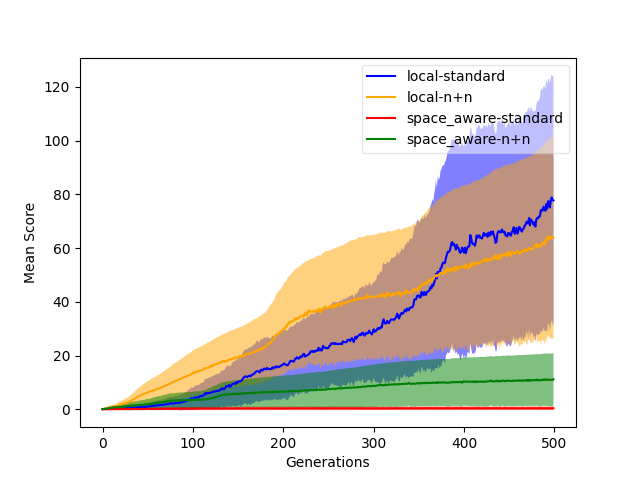
\includegraphics[width=1\linewidth]{all}
    \caption{All algorithm variants compared over 500 gens}
    \label{all}
  \end{minipage}%
  \begin{minipage}{.5\textwidth}
    \centering
    \captionsetup{width=.8\linewidth}
    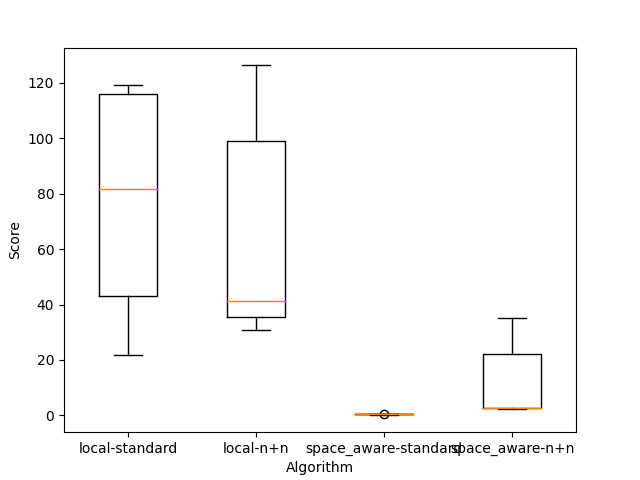
\includegraphics[width=1\linewidth]{box}
    \caption{Boxplot of final generation for each algorithm variant}
    \label{box}
  \end{minipage}
\end{figure}

\subsection{Effects of Changing Evolutionary Selection Method}

Figure \ref{local} compares standard evolution to n+n for local collision sensing, while \verb|local-standard| was the prevailing algorithm after 500 generations, \verb|local-n+n| is consistently performs better from generation 0 until a crossover point at approximately 50 score. Average Mann-Whitney-U and difference of means are:
$$
U = 32.8, p = 0.39137, m = 8.9
$$
As $p > 0.05$, changing evolution selection methods for local sensing is not statistically significant.
\bigskip

Figure \ref{space_aware} compares standard to n+n evolution for space aware collision sensing. As shown in the graph, n+n performed significantly better than standard evolution, though standard deviation was large. Standard evolution struggled to make any progress throughout generations, with a consistently average score throughout generations of 0. Average Mann-Whitney-U and difference of means are:
$$
U = 0.0, p = 0.00018, m = 6.7
$$
Changing evolution selection methods for space aware sensing is statistically significant as $p < 0.05$. While the difference of means $m$ does not immediately suggest a large effect size, when considering figure \ref{space_aware} the data shows that n+n evolution allows space aware sensing to be a viable collision detection method unlike standard evolution. This is likely due to n+n evolution being significantly more sensitive to marginal improvements in fitness within a generation, as n+n is designed to preserve best individuals, while standard evolution leaves the survival of an individual down to a weighted probability.

\begin{figure}[h]
  \centering
  \begin{minipage}{.5\textwidth}
    \centering
    \captionsetup{width=.8\linewidth}
    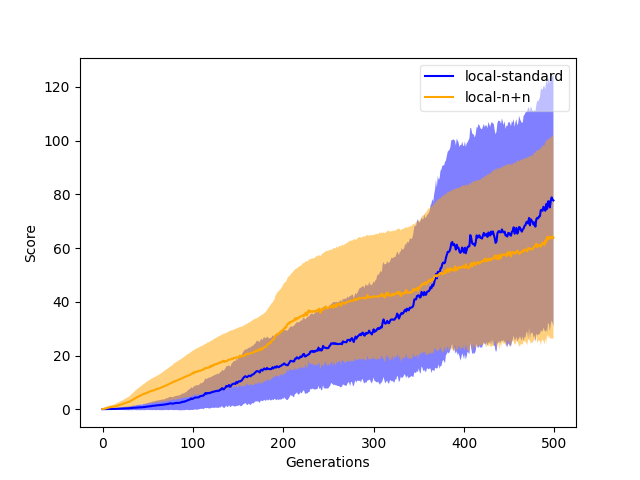
\includegraphics[width=1 \linewidth]{local}
    \caption{\texttt{local-standard} compared to \texttt{local-n+n} over 500 gens}
    \label{local}
  \end{minipage}%
  \begin{minipage}{.5\textwidth}
    \centering
    \captionsetup{width=.8\linewidth}
    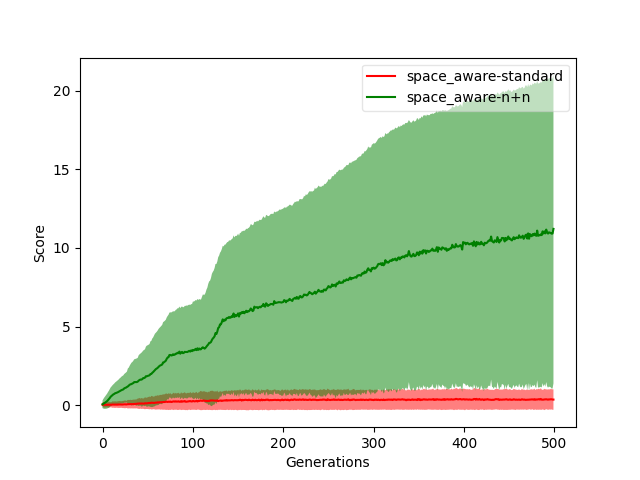
\includegraphics[width=1\linewidth]{space_aware}
    \caption{\texttt{space\_aware-standard} compared to \texttt{space\_aware-n+n} over 500 gens}
    \label{space_aware}
  \end{minipage}
\end{figure}


\subsection{Effects of Changing Collision Sensing Method}

Figure \ref{standard} compares local collision sensing to space aware collision sensing using standard evolution. Local collision sensing managed to successfully learn how to achieve high scores, with best individuals even able to complete the game by filling every square. Space aware collision sensing was unsuccessful in any of the 10 runs to evolve any sustainable method of finding food and increasing score. Average Mann-Whitney-U and difference of means are:
$$
U = 0.2, p = 0.00063, m = 28.7
$$
As $p < 0.05$, these results are statistically significant. This is due to \verb|space_aware-standard| not successfully evolving any method of increasing score, while \verb|local-standard| was extremely successful. An average difference of means of 28.7 combined with a $U$ value of 0.2 shows a large effect size.
\bigskip

Figure \ref{n+n} compares also compares local collision sensing to space aware collision sensing, however n+n evolution is used to evolve the population.  Average Mann-Whitney-U and difference of means are:
$$
U = 9.0, p = 0.00404, m = 26.5
$$

These results are statistically significant ($p < 0.05$). In contrast to figure \ref{standard}, n+n evolution has successfully trained space aware collision to be able to achieve a non-zero average score. Regardless of this, space aware collision sensing still performed significantly worse than local sensing, with an average difference of means of 26.5. The effect size of this statistical comparison is large, as evidenced by a $U$ value of 9.0. These difference of means and $U$ value are influenced by early generations, however local sensing quickly outperforms space aware sensing as evidenced in figure \ref{n+n}.

\begin{figure}[h]
  \centering
  \begin{minipage}{.5\textwidth}
    \centering
    \captionsetup{width=.8\linewidth}
    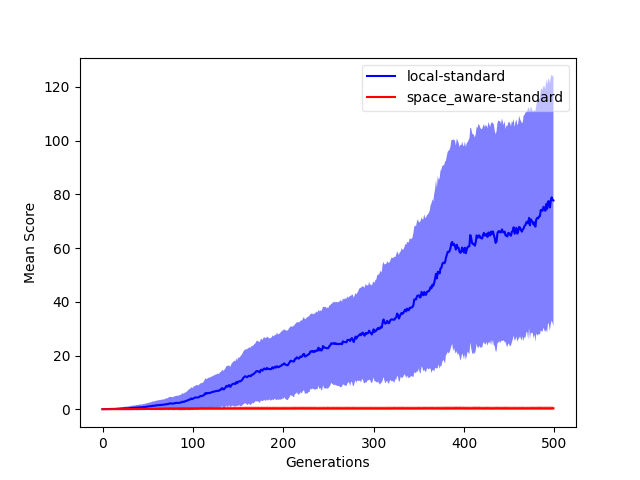
\includegraphics[width=1\linewidth]{standard}
    \caption{\texttt{local-standard} compared to \texttt{space\_aware-standard} over 500 gens}
    \label{standard}
  \end{minipage}%
  \begin{minipage}{.5\textwidth}
    \centering
    \captionsetup{width=.8\linewidth}
    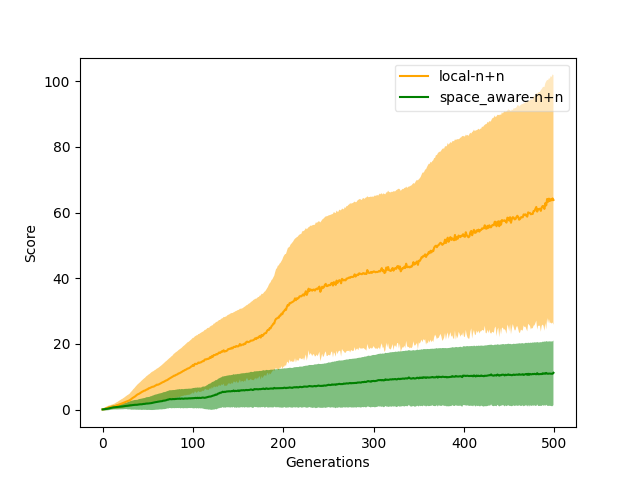
\includegraphics[width=1\linewidth]{n+n}
    \caption{\texttt{local-n+n} compared to \texttt{space\_aware-n+n} over 500 gens}
    \label{n+n}
  \end{minipage}
\end{figure}





